Uma vez pré-processados os dados dos sensores procedeu-se a realizar a calibração das leituras de \acrshort{co}, \acrshort{o3} e \acrshort{mp}, utilizando como referência os dados provenientes de uma estação de monitoramento de qualidade do ar. Foram explorados diferentes modelos multivariados para a calibração, i.e.: o Perceptron Multicamadas (MLP), Regressão Linear Multivariada (MLR), K Vizinhos mais Próximos (KNN) e as Florestas Aleatórias (RF). A escolha desses modelos baseou-se na capacidade de lidar com múltiplas variáveis simultaneamente, proporcionando uma adaptação mais eficaz às complexidades das relações entre os dados dos sensores e as condições ambientais de temperatura.

A calibração foi realizada em duas fases. Inicialmente, considerou-se apenas os dados do sensor em questão e a temperatura como variáveis de entrada. Para encontrar o modelo que melhor explicasse os dados foi realizada uma busca em \textit{grid} que combina diferentes parâmetros e variáveis de entrada e avalia cada modelo utilizando validações cruzadas com k = 3 Posteriormente, expandiu-se o escopo para incluir os dados de outros sensores disponíveis. Essa abordagem permitiu avaliar o impacto da inclusão de mais variáveis na precisão da calibração. A avaliação comparativa dos modelos de calibração foi realizada mediante métricas essenciais, incluindo o coeficiente de determinação (r2), o erro médio quadrático (RMSE) e o erro absoluto médio (MAE). A utilização de validações cruzadas proporciona uma análise mais robusta e imparcial do desempenho dos modelos.

A expectativa é que a implementação desses modelos de calibração aprimore significativamente a qualidade dos dados, fornecendo uma base sólida para análises subsequentes relacionadas à qualidade do ar. Os resultados desta pesquisa têm o potencial não apenas de beneficiar a precisão dos dados locais, mas também de contribuir para o desenvolvimento de metodologias aprimoradas de calibração em ambientes de monitoramento ambiental.

\subsection{Calibração das leituras do sensor CO-B4}

Nas Figuras \ref{fig:data-co-reference-time-series} e \ref{fig:data-co-reference-corr} apresentam-se as leituras de \acrshort{co} obtidas pelo sensor CO-B4 de Alphasense e a estação de referência. Observa-se que as leituras do sensor CO-B4 em geral subestimaram os valores de concentração de referência. Os testes de Spearman e Kendall revelaram a existência de correlação entre as medições com o sensor de baixo custo e a referência com coeficientes de 0.3 e 0.2 respectivamente.

\begin{figure}[h]
    \centering
    \caption{Séries temporais e gráficos de dispersão das medições de \acrshort{co}}
    \begin{subfigure}{0.495\textwidth}
        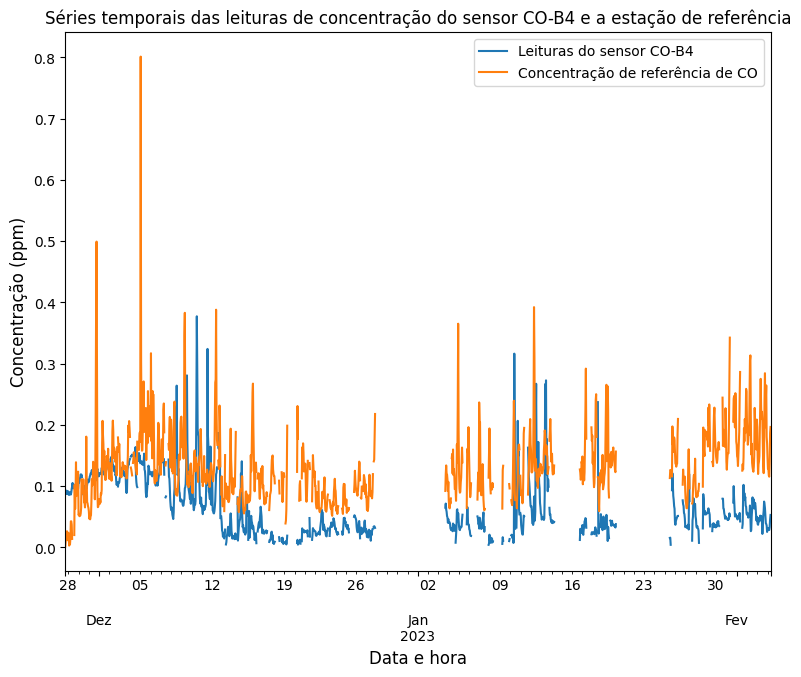
\includegraphics[width=\textwidth]{chapters/3-RESULTADOS CAMPO/Figuras/co-b4-reference-time-series.png}
        \caption{Séries temporais das leituras do sensor CO-B4 e a estação de referência}
        \label{fig:data-co-reference-time-series}
    \end{subfigure}
    \hfill
    \begin{subfigure}{0.495\textwidth}
        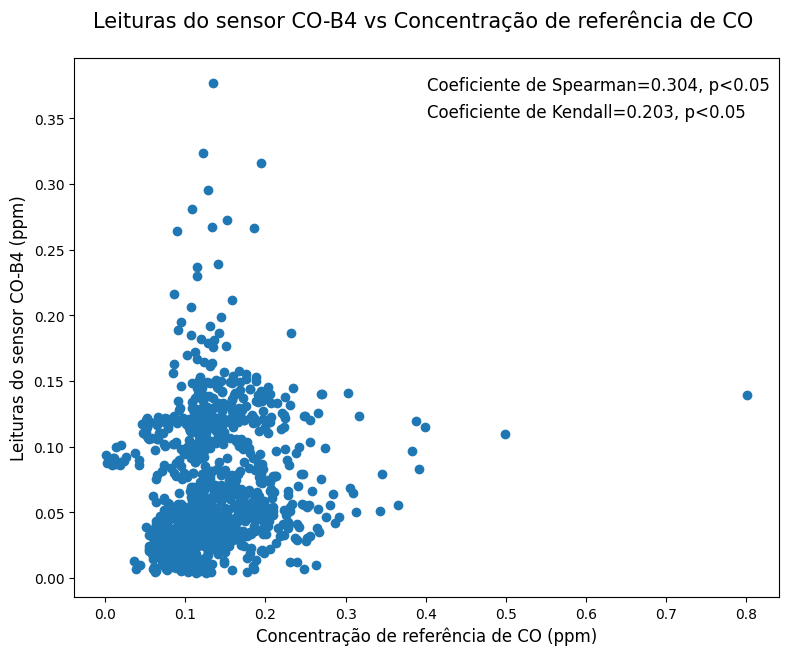
\includegraphics[width=\textwidth]{chapters/3-RESULTADOS CAMPO/Figuras/co-b4-reference-correlation.png}
        \caption{Gráfico de dispersão das leituras do sensor CO-B4 e a estação de referência}
        \label{fig:data-co-reference-corr}
    \end{subfigure}
    \fonte{Desenvolvido pelo autor (2023)}
\end{figure}

\subsubsection{Calibração utilizando as leituras do sensor CO-B4 e a temperatura}

Na Tabela \ref{tab:data-co-br-calib-results} resumem-se os melhores modelos encontrados pela busca em \textit{grid} para calibrar as leituras do sensor CO-B4. A Figura \ref{fig:data-co-b4-models-performance} apresenta o desempenho dos modelos e as variáveis de entrada considerando os valores de r2, RMSE e MAE.

\begin{table}[h]
    \caption{Resultados da calibração do sensor CO-B4}
    \centering
    \begin{tabularx}{0.95\textwidth}[h]{
         >{\raggedright\hsize=.08\hsize\arraybackslash}X
         >{\raggedright\hsize=.8\hsize\arraybackslash}X 
         >{\raggedright\hsize=.5\hsize\arraybackslash}X
         >{\raggedright\hsize=.5\hsize\arraybackslash}X 
         >{\raggedright\hsize=.5\hsize\arraybackslash}X }
        \hline
        Var. & Modelo & R2 & RMSE & MAE\\ [0.5ex]
        \hline
        CO & \textbf{MLP}: & -0.64 ± 0.49 & -0.07 ± 0.01 & -0.05 \\ [0.5ex]
           & alpha = 0.01 &  & & \\ [0.5ex]
           & hidden layers = (200, 10) & & & \\ [0.5ex]
           & & & & \\ [0.5ex]
           & \textbf{MLR} & -0.61 ± 0.47 & -0.07 ± 0.01 & -0.05 \\ [0.5ex]
           & & & & \\ [0.5ex]
           & \textbf{KNN:} & -0.47 ± 0.29 & -0.06 ± 0.01 & -0.05 \\ [0.5ex]
           & n\_neighbors = 17 & & & \\ [0.5ex]
           & weights = uniform & & & \\ [0.5ex]
           & & & & \\ [0.5ex]
           & \textbf{RF:} & -0.60 ± 0.34 & -0.07 ± 0.01 & -0.05 \\ [0.5ex]
           & max\_depth = 30 & & & \\ [0.5ex]
           & min\_samples\_leaf = 4 & & & \\ [0.5ex]
           & min\_samples\_split = 10 & & & \\ [0.5ex]
           & n\_estimators = 150 & & & \\ [0.5ex]
        \hline
        CO, T & \textbf{MLP:} & -0.59 ± 0.42 & -0.07 ± 0.01 & -0.05 \\ [0.5ex]
              & alpha = 0.1 & & & \\ [0.5ex]
              & hidden layer = (200, 50) & & & \\ [0.5ex]
              & & & & \\ [0.5ex]
              & \textbf{MLR:} & -0.65 ± 0.45 & -0.07 ± 0.01 & -0.05 \\ [0.5ex]
              & & & & \\ [0.5ex]
              & \textbf{KNN:} & -0.61 ± 0.46 & -0.07 ± 0.01 & -0.05 \\ [0.5ex]
              & n\_neighbors = 15 & & & \\ [0.5ex]
              & weights = uniform & & & \\ [0.5ex]
              & & & & \\ [0.5ex]
              & \textbf{RF:} & -0.72 +/- 0.50 & -0.07 ± 0.01 & -0.05 \\ [0.5ex]
              & max\_depth = None & & & \\ [0.5ex]
              & min\_samples\_leaf = 4 & & & \\ [0.5ex]
              & min\_samples\_split = 2 & & & \\ [0.5ex]
              & n\_estimators = 100 & & & \\ [0.5ex]
        \hline
    \end{tabularx}
    \label{tab:data-co-br-calib-results}
    \fonte{Desenvolvido pelo autor}
\end{table}

\begin{figure}[h]
    \centering
    \caption{Resultados dos modelos de calibração aplicados as leituras do sensor CO-B4}
    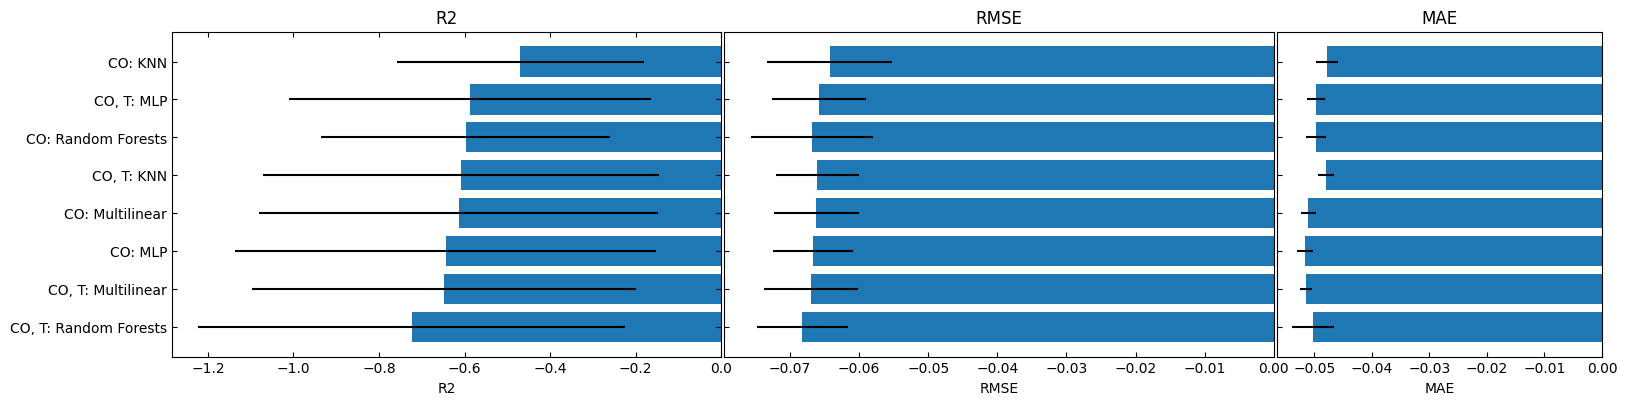
\includegraphics[width=\textwidth]{chapters/3-RESULTADOS CAMPO/Figuras/co-b4-models-performance.png}
    \label{fig:data-co-b4-models-performance}
    \fonte{Desenvolvido pelo autor (2023)}
\end{figure}

\subsection{Calibração das leituras dos sensores OX-B431}

Nas Figuras \ref{fig:data-o3-reference-time-series}, \ref{fig:data-o3-1-reference-corr} e \ref{fig:data-o3-2-reference-corr} apresentam-se as leituras de \acrshort{o3} obtidas pelos sensores OX-B431 de Alphasense e a estação de referência. Observa-se que as leituras do sensor OX-B431 em geral superestimaram os valores de concentração de referência. Os testes de Spearman e Kendall revelaram a existência de correlação entre as medições com o sensor de baixo custo e a referência com coeficientes de 0.3 e 0.2 respectivamente.

\begin{figure}[h]
    \centering
    \caption{Séries temporais e gráficos de dispersão das medições de \acrshort{o3}}
    \begin{subfigure}{0.99\textwidth}
        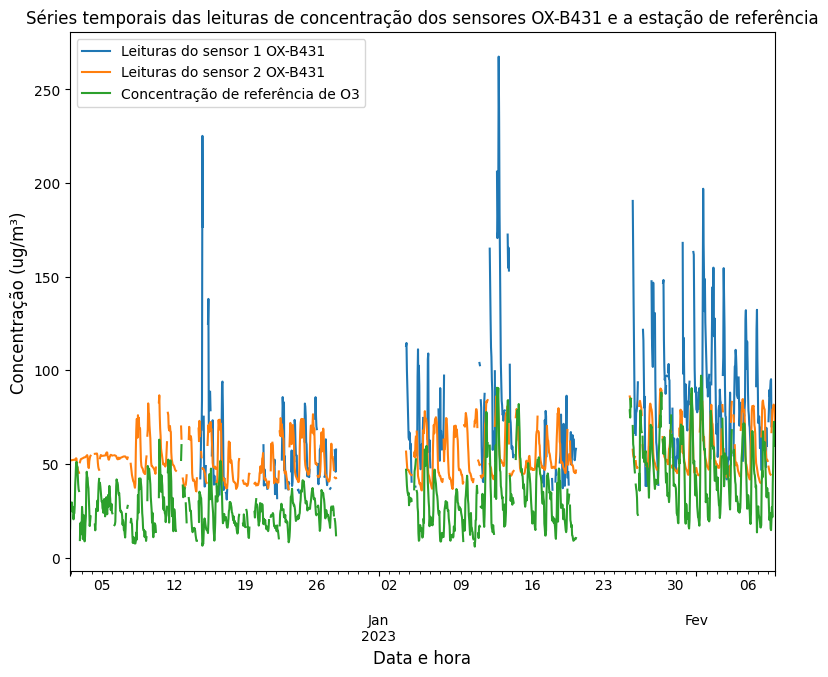
\includegraphics[width=\textwidth]{chapters/3-RESULTADOS CAMPO/Figuras/o3-b4-reference-time-series.png}
        \caption{Séries temporais das leituras dos sensores OX-B431 e a estação de referência}
        \label{fig:data-o3-reference-time-series}
    \end{subfigure}
    \hfill
    \begin{subfigure}{0.495\textwidth}
        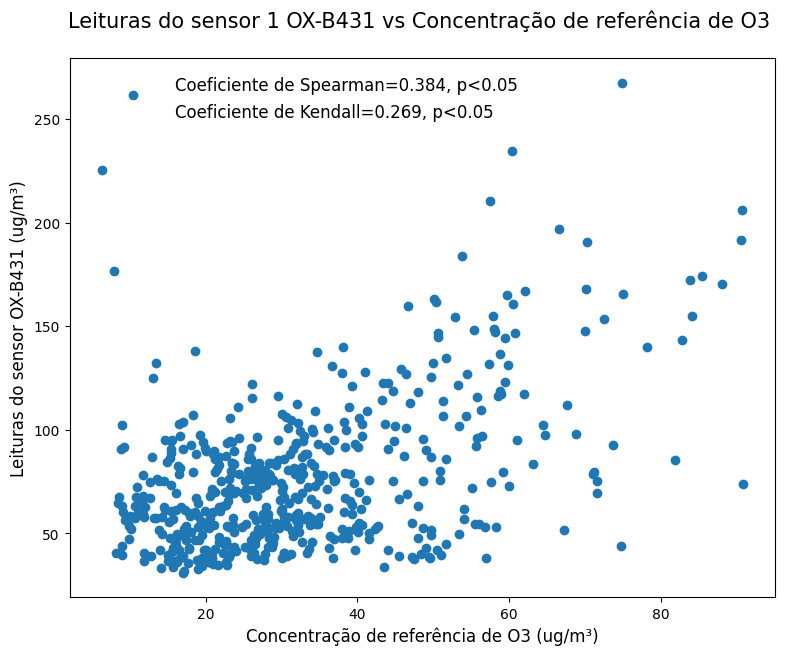
\includegraphics[width=\textwidth]{chapters/3-RESULTADOS CAMPO/Figuras/o3-b4-1-reference-correlation.png}
        \caption{Gráfico de dispersão das leituras do sensor 1 OX-B431 e a estação de referência}
        \label{fig:data-o3-1-reference-corr}
    \end{subfigure}
    \hfill
    \begin{subfigure}{0.495\textwidth}
        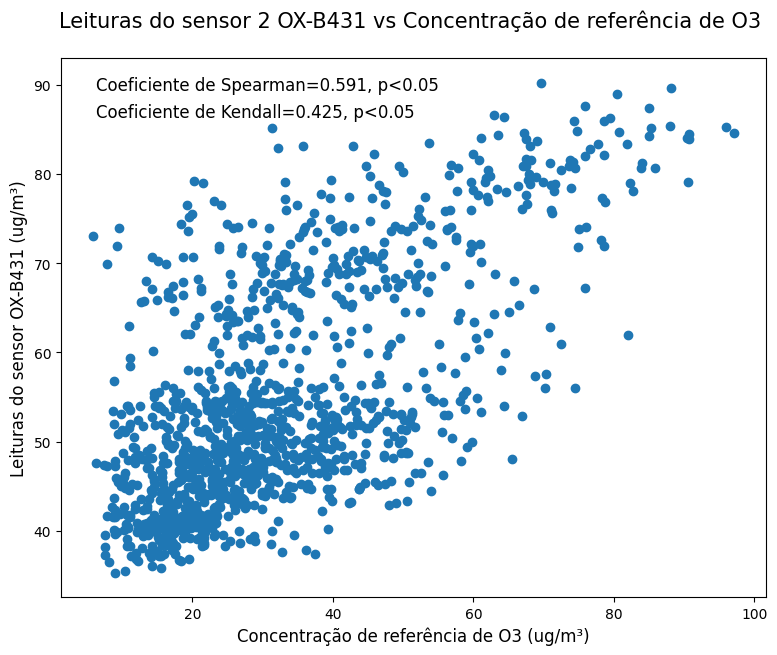
\includegraphics[width=\textwidth]{chapters/3-RESULTADOS CAMPO/Figuras/o3-b4-2-reference-correlation.png}
        \caption{Gráfico de dispersão das leituras do sensor 2 OX-B431 e a estação de referência}
        \label{fig:data-o3-2-reference-corr}
    \end{subfigure}
    \fonte{Desenvolvido pelo autor (2023)}
\end{figure}

\subsubsection{Calibração utilizando as leituras dos sensores OX-B431 e a temperatura}

Na Tabela \ref{tab:data-o3-b4-calib-results} resumem-se os melhores modelos encontrados pela busca em \textit{grid} para calibrar as leituras do sensor OX-B431. A Figura \ref{fig:data-o3-b4-models-performance} apresenta o desempenho dos modelos e as variáveis de entrada considerando os valores de r2, RMSE e MAE.

\begin{table}[h]
    \caption{Resultados da calibração dos sensores OX-B431}
    \centering
    \begin{tabularx}{0.95\textwidth}[h]{
         >{\raggedright\hsize=.08\hsize\arraybackslash}X
         >{\raggedright\hsize=.8\hsize\arraybackslash}X 
         >{\raggedright\hsize=.5\hsize\arraybackslash}X
         >{\raggedright\hsize=.5\hsize\arraybackslash}X 
         >{\raggedright\hsize=.5\hsize\arraybackslash}X }
        \hline
        Var. & Modelo & R2 & RMSE & MAE\\ [0.5ex]
        \hline
        O3 & \textbf{MLP}: & -0.64 ± 0.49 & -0.07 ± 0.01 & -0.05 \\ [0.5ex]
           & alpha = 0.01 &  & & \\ [0.5ex]
           & hidden layers = (200, 10) & & & \\ [0.5ex]
           & & & & \\ [0.5ex]
           & \textbf{MLR} & -0.61 ± 0.47 & -0.07 ± 0.01 & -0.05 \\ [0.5ex]
           & & & & \\ [0.5ex]
           & \textbf{KNN:} & -0.47 ± 0.29 & -0.06 ± 0.01 & -0.05 \\ [0.5ex]
           & n\_neighbors = 17 & & & \\ [0.5ex]
           & weights = uniform & & & \\ [0.5ex]
           & & & & \\ [0.5ex]
           & \textbf{RF:} & -0.60 ± 0.34 & -0.07 ± 0.01 & -0.05 \\ [0.5ex]
           & max\_depth = 30 & & & \\ [0.5ex]
           & min\_samples\_leaf = 4 & & & \\ [0.5ex]
           & min\_samples\_split = 10 & & & \\ [0.5ex]
           & n\_estimators = 150 & & & \\ [0.5ex]
        \hline
        O3, T & \textbf{MLP:} & -0.59 ± 0.42 & -0.07 ± 0.01 & -0.05 \\ [0.5ex]
              & alpha = 0.1 & & & \\ [0.5ex]
              & hidden layer = (200, 50) & & & \\ [0.5ex]
              & & & & \\ [0.5ex]
              & \textbf{MLR:} & -0.65 ± 0.45 & -0.07 ± 0.01 & -0.05 \\ [0.5ex]
              & & & & \\ [0.5ex]
              & \textbf{KNN:} & -0.61 ± 0.46 & -0.07 ± 0.01 & -0.05 \\ [0.5ex]
              & n\_neighbors = 15 & & & \\ [0.5ex]
              & weights = uniform & & & \\ [0.5ex]
              & & & & \\ [0.5ex]
              & \textbf{RF:} & -0.72 +/- 0.50 & -0.07 ± 0.01 & -0.05 \\ [0.5ex]
              & max\_depth = None & & & \\ [0.5ex]
              & min\_samples\_leaf = 4 & & & \\ [0.5ex]
              & min\_samples\_split = 2 & & & \\ [0.5ex]
              & n\_estimators = 100 & & & \\ [0.5ex]
        \hline
    \end{tabularx}
    \label{tab:data-o3-b4-calib-results}
    \fonte{Desenvolvido pelo autor}
\end{table}

\begin{figure}[h]
    \centering
    \caption{Resultados dos modelos de calibração aplicados às leituras dos sensores OX-B431}
    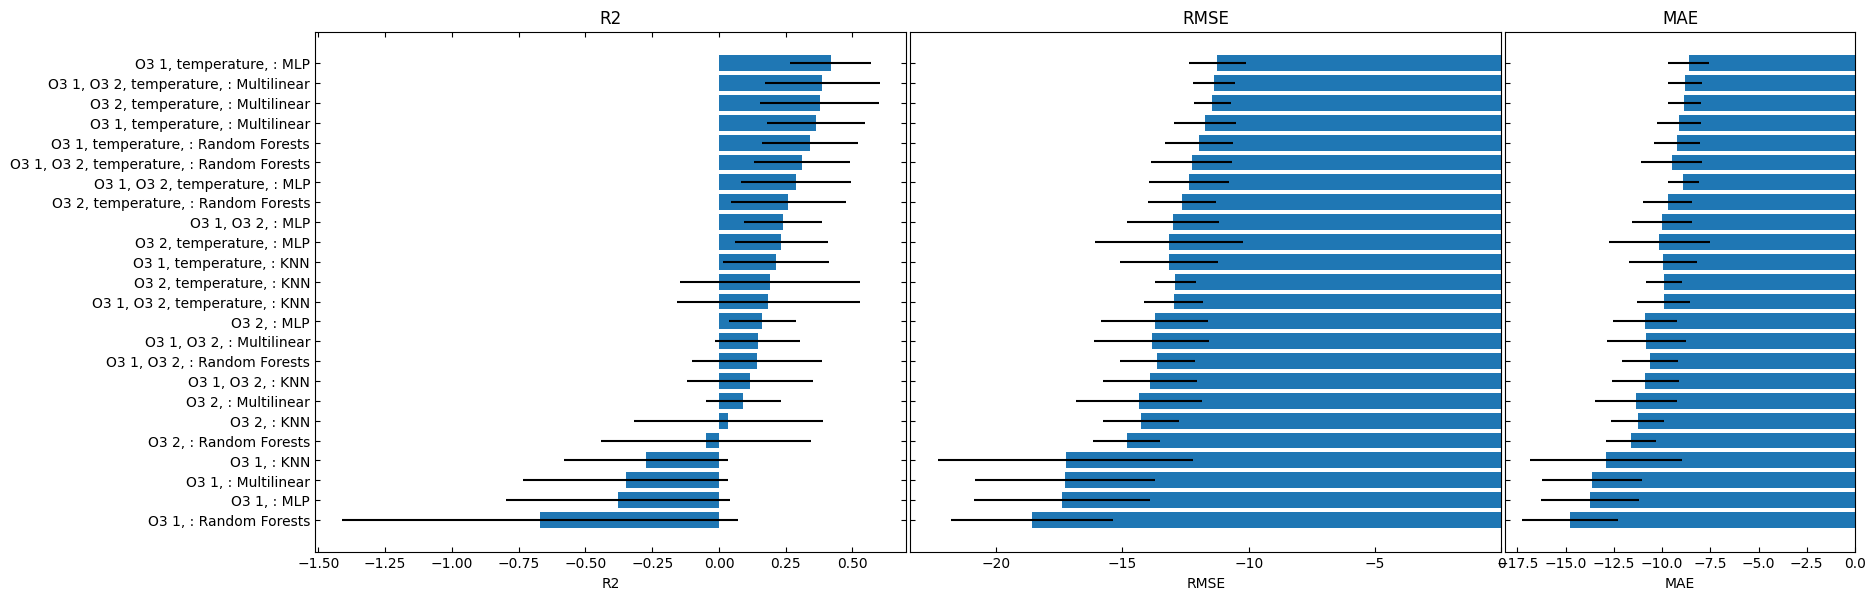
\includegraphics[width=\textwidth]{chapters/3-RESULTADOS CAMPO/Figuras/o3-b4-models-performance.png}
    \label{fig:data-o3-b4-models-performance}
    \fonte{Desenvolvido pelo autor (2023)}
\end{figure}

\subsection{Calibração das leituras de \acrshort{mp10} do sensor OPC-N3}

Nas Figuras \ref{fig:data-pm10-reference-time-series} e \ref{fig:data-pm10-reference-corr} apresentam-se as leituras de \acrshort{mp10} obtidas pelo sensor OPC-N3 de Alphasense e a estação de referência. Observa-se que as leituras do sensor OPC-N3 em geral subestimaram os valores de concentração de referência. Os testes de Spearman e Kendall revelaram a existência de correlação entre as medições com o sensor de baixo custo e a referência com coeficientes de 0.3 e 0.2 respectivamente.

\begin{figure}[h]
    \centering
    \caption{Séries temporais e gráficos de dispersão das medições de \acrshort{mp10}}
    \begin{subfigure}{0.495\textwidth}
        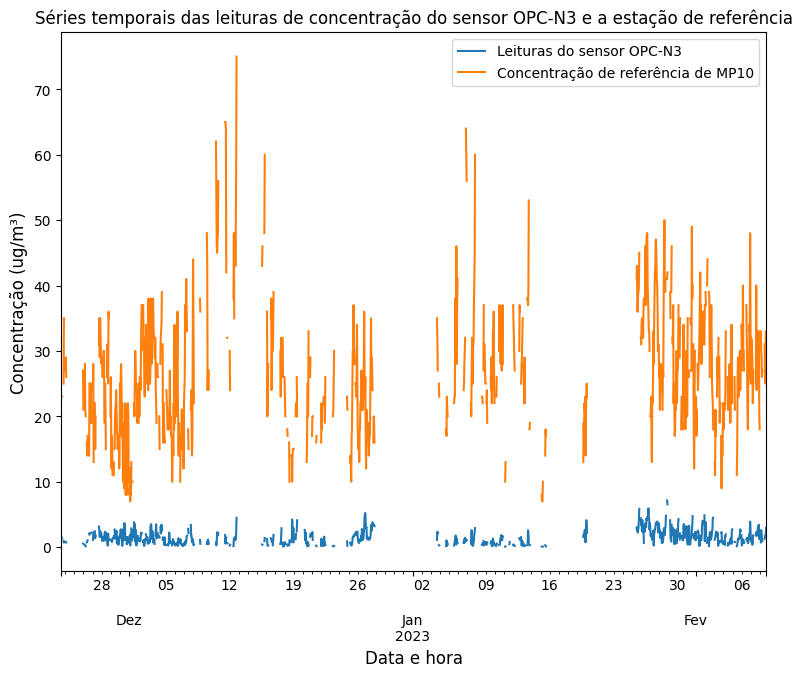
\includegraphics[width=\textwidth]{chapters/3-RESULTADOS CAMPO/Figuras/pm10-reference-time-series.png}
        \caption{Séries temporais das leituras de \acrshort{mp10} do sensor OPC-N3 e a estação de referência}
        \label{fig:data-pm10-reference-time-series}
    \end{subfigure}
    \hfill
    \begin{subfigure}{0.495\textwidth}
        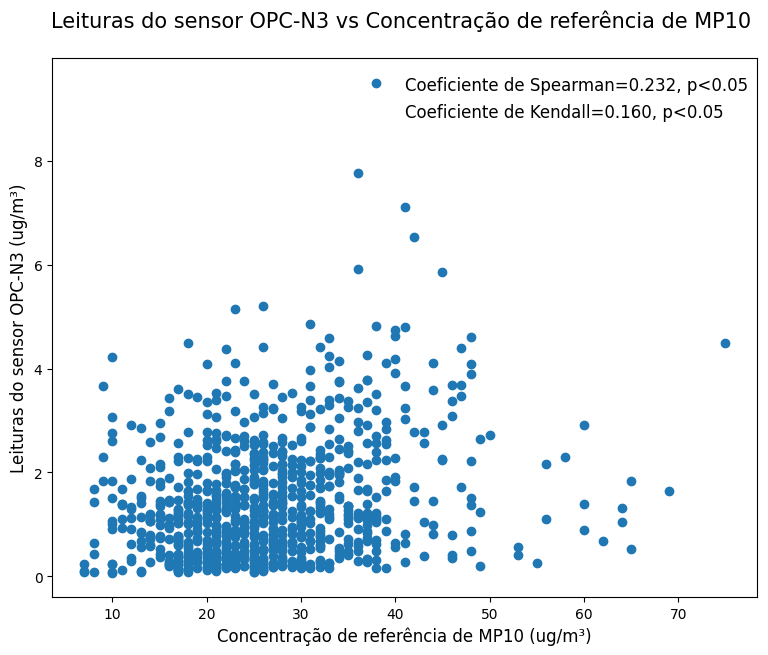
\includegraphics[width=\textwidth]{chapters/3-RESULTADOS CAMPO/Figuras/pm10-reference-correlation.png}
        \caption{Gráfico de dispersão das leituras de \acrshort{mp10} do sensor OPC-N3 e a estação de referência}
        \label{fig:data-pm10-reference-corr}
    \end{subfigure}
    \fonte{Desenvolvido pelo autor (2023)}
\end{figure}

\subsubsection{Calibração utilizando as leituras de \acrshort{mp10}do sensor OPC-N3 e a temperatura}

Na Tabela \ref{tab:data-pm10-calib-results} resumem-se os melhores modelos encontrados pela busca em \textit{grid} para calibrar as leituras de \acrshort{mp10} do sensor OPC-N3. A Figura \ref{fig:data-pm10-models-performance} apresenta o desempenho dos modelos e as variáveis de entrada considerando os valores de r2, RMSE e MAE.

\begin{table}[h]
    \caption{Resultados da calibração das leituras de \acrshort{mp10} do sensor OPC-N3}
    \centering
    \begin{tabularx}{0.95\textwidth}[h]{
         >{\raggedright\hsize=.08\hsize\arraybackslash}X
         >{\raggedright\hsize=.8\hsize\arraybackslash}X 
         >{\raggedright\hsize=.5\hsize\arraybackslash}X
         >{\raggedright\hsize=.5\hsize\arraybackslash}X 
         >{\raggedright\hsize=.5\hsize\arraybackslash}X }
        \hline
        Var. & Modelo & R2 & RMSE & MAE\\ [0.5ex]
        \hline
        CO & \textbf{MLP}: & -0.64 ± 0.49 & -0.07 ± 0.01 & -0.05 \\ [0.5ex]
           & alpha = 0.01 &  & & \\ [0.5ex]
           & hidden layers = (200, 10) & & & \\ [0.5ex]
           & & & & \\ [0.5ex]
           & \textbf{MLR} & -0.61 ± 0.47 & -0.07 ± 0.01 & -0.05 \\ [0.5ex]
           & & & & \\ [0.5ex]
           & \textbf{KNN:} & -0.47 ± 0.29 & -0.06 ± 0.01 & -0.05 \\ [0.5ex]
           & n\_neighbors = 17 & & & \\ [0.5ex]
           & weights = uniform & & & \\ [0.5ex]
           & & & & \\ [0.5ex]
           & \textbf{RF:} & -0.60 ± 0.34 & -0.07 ± 0.01 & -0.05 \\ [0.5ex]
           & max\_depth = 30 & & & \\ [0.5ex]
           & min\_samples\_leaf = 4 & & & \\ [0.5ex]
           & min\_samples\_split = 10 & & & \\ [0.5ex]
           & n\_estimators = 150 & & & \\ [0.5ex]
        \hline
        CO, T & \textbf{MLP:} & -0.59 ± 0.42 & -0.07 ± 0.01 & -0.05 \\ [0.5ex]
              & alpha = 0.1 & & & \\ [0.5ex]
              & hidden layer = (200, 50) & & & \\ [0.5ex]
              & & & & \\ [0.5ex]
              & \textbf{MLR:} & -0.65 ± 0.45 & -0.07 ± 0.01 & -0.05 \\ [0.5ex]
              & & & & \\ [0.5ex]
              & \textbf{KNN:} & -0.61 ± 0.46 & -0.07 ± 0.01 & -0.05 \\ [0.5ex]
              & n\_neighbors = 15 & & & \\ [0.5ex]
              & weights = uniform & & & \\ [0.5ex]
              & & & & \\ [0.5ex]
              & \textbf{RF:} & -0.72 +/- 0.50 & -0.07 ± 0.01 & -0.05 \\ [0.5ex]
              & max\_depth = None & & & \\ [0.5ex]
              & min\_samples\_leaf = 4 & & & \\ [0.5ex]
              & min\_samples\_split = 2 & & & \\ [0.5ex]
              & n\_estimators = 100 & & & \\ [0.5ex]
        \hline
    \end{tabularx}
    \label{tab:data-pm10-calib-results}
    \fonte{Desenvolvido pelo autor}
\end{table}

\begin{figure}[h]
    \centering
    \caption{Resultados dos modelos de calibração aplicados as leituras de \acrshort{mp10} do sensor OPC-N3}
    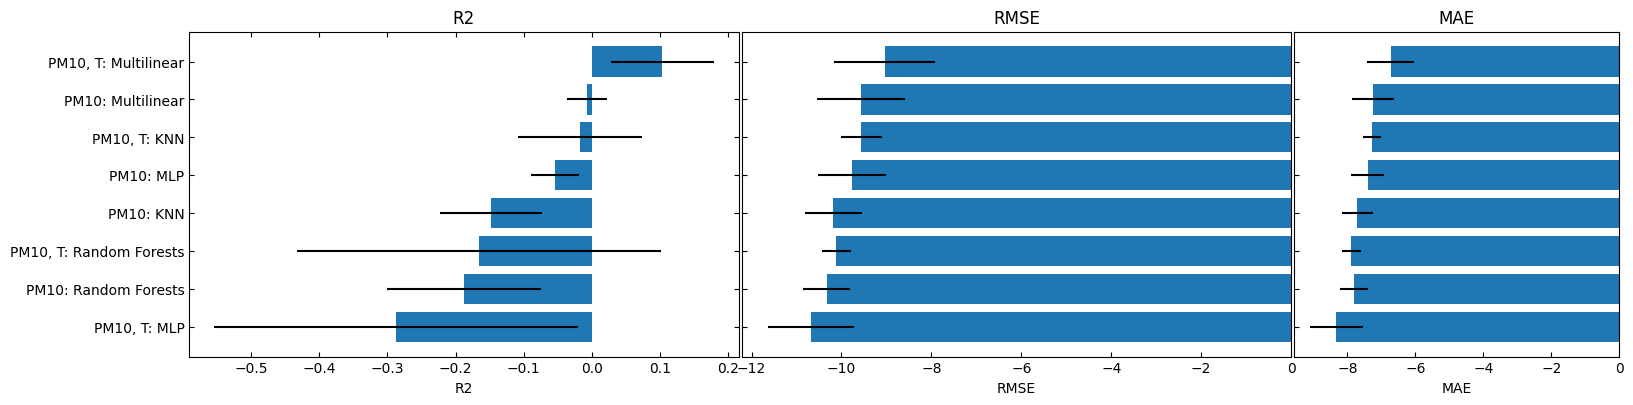
\includegraphics[width=\textwidth]{chapters/3-RESULTADOS CAMPO/Figuras/pm10-models-performance.png}
    \label{fig:data-pm10-models-performance}
    \fonte{Desenvolvido pelo autor (2023)}
\end{figure}
